\documentclass[11pt,french]{beamer}

\usepackage[utf8]{inputenc}
\usepackage[T1]{fontenc}
\usepackage[french]{babel}
\usepackage{graphicx}
\usepackage{booktabs}
\usepackage{array}
\usepackage{tabularx}
\usepackage{multicol}
\usepackage{hyperref}
\usepackage{tikz}
\usetikzlibrary{arrows.meta, positioning, fit, calc, backgrounds}

\usetheme{Madrid}
\usecolortheme{whale}
\useinnertheme{rounded}

\definecolor{uyblue}{RGB}{0,102,153}
\definecolor{uyblueDark}{RGB}{0,70,110}
\definecolor{uygray}{RGB}{245,245,245}

\setbeamercolor{structure}{fg=uyblue}
\setbeamercolor{frametitle}{bg=uyblue,fg=white}
\setbeamercolor{title}{fg=uyblueDark}
\setbeamercolor{block title}{bg=uyblue,fg=white}
\setbeamercolor{block body}{bg=uygray,fg=black}

\setbeamertemplate{navigation symbols}{}
\setbeamertemplate{footline}{
  \hfill
  \usebeamercolor[fg]{author in head/foot}
  \insertframenumber{} / \inserttotalframenumber
  \hspace{1em}
  \vspace{0.5em}
}

\title[Système FL distribué]{Système distribué d'apprentissage fédéré}
\subtitle{INF4218 — Programmation Distribuée}
\author[MFENJOU et al.]{
  MFENJOU ANAS CHERIF (21T2330) \\
  EDU GUIEDI HERMANN ARNOLD (22T2876) \\
  LANGOUL FADILA MARIAMA MOUNIRA (21T2528)
}
\institute[UY1]{
  Université de Yaoundé I \\
  Faculté des Sciences — Département d'Informatique \\
  Master I Systèmes et Réseaux \\
  Année académique 2025–2026
}
\date{Juin 2026}
\titlegraphic{
\includegraphics[height=1.6cm]{assets/logo_uy1.png}}

\begin{document}

% ============================================================
\begin{frame}
  \titlepage
\end{frame}

% ============================================================
\begin{frame}{Plan}
  \tableofcontents
\end{frame}

% ============================================================
\section{Introduction}

\begin{frame}{Contexte et objectifs}
  \begin{block}{Cadre du projet}
    Travail pratique \textbf{INF4218 — Programmation Distribuée} \\
    Référence : Van Steen \& Tanenbaum, \textit{Distributed Systems}, ch.~1 à 8
  \end{block}

  \textbf{Objectif :} concevoir un \textbf{système distribué d'apprentissage fédéré}
  (*Federated Learning*) mettant en \oe uvre l'ensemble des concepts obligatoires du cours.

  \vspace{0.3cm}
  \begin{itemize}
    \item Clients : entraînement \textbf{local} sur données privées
    \item Serveur : \textbf{agrégation} des gradients $\rightarrow$ modèle global
    \item Illustration : coordination, RPC, cohérence temporelle, tolérance aux pannes
  \end{itemize}

  \vspace{0.2cm}
  \small\textbf{Stack :} Python 3.14, gRPC/Protobuf, NumPy, pytest \\
  \small\textbf{Dépôt :} \url{https://github.com/CherifMfenjou/INF4218-TPSD}
\end{frame}

\begin{frame}{Concepts obligatoires implémentés}
  \small
  \begin{tabular}{@{}ll@{}}
    \toprule
    \textbf{Concept} & \textbf{Chapitre Tanenbaum} \\
    \midrule
    Architecture client-serveur multi-niveaux & 2 \\
    Nommage plat / structuré / par attributs & 6.2 -- 6.4 \\
    Horloges logiques de Lamport & 5.2.1 \\
    Élection de leader (Bully) & 5.4.1 \\
    Exclusion mutuelle distribuée (Ricart-Agrawala) & 5.3.3 \\
    Communication RPC / gRPC & 4 \\
    Tolérance aux pannes (checkpoint / recovery) & 8.6.2 \\
    \bottomrule
  \end{tabular}

  \vspace{0.6cm}
  \begin{center}
    \textbf{41 tests} (40 unitaires + 1 intégration) --- \textbf{tous passent}
  \end{center}
\end{frame}

% ============================================================
\section{Conception}

\begin{frame}{Architecture globale du système}
  \centering
  \vspace{-0.35cm}
  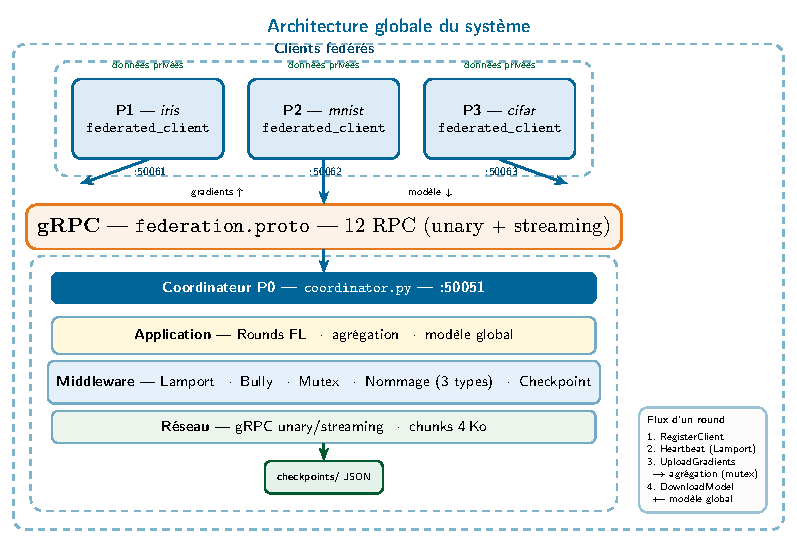
\includegraphics[width=\linewidth,height=0.82\textheight,keepaspectratio]{assets/architecture-du-projet.pdf}
\end{frame}

\begin{frame}{Architecture à trois niveaux}
  \begin{columns}[T]
    \column{0.48\textwidth}
    \begin{block}{Couche Application}
      Rounds FL, entraînement local, agrégation fédérée
    \end{block}
    \begin{block}{Couche Middleware}
      Lamport, Bully, mutex, nommage, checkpoint
    \end{block}
    \begin{block}{Couche Réseau (gRPC)}
      RPC unary + streaming
    \end{block}

    \column{0.48\textwidth}
    \textbf{Serveur} \texttt{FederationCoordinator} (P0)
    \begin{itemize}\small
      \item Coordination des rounds et modèle global
      \item Registres de nommage (3 paradigmes)
      \item Checkpoints et recovery
    \end{itemize}

    \vspace{0.2cm}
    \textbf{Clients} \texttt{FederatedClient} (P1, P2, P3\ldots)
    \begin{itemize}\small
      \item Inscription (\texttt{RegisterClient})
      \item Entraînement local et échange de gradients
      \item Heartbeats périodiques
    \end{itemize}
  \end{columns}
\end{frame}

\begin{frame}{Flux d'un round d'apprentissage fédéré}
  \small
  \begin{center}
    \begin{tabular}{@{}c c@{}}
      \textbf{Client} & \textbf{Coordinateur} \\[0.3em]
      \multicolumn{2}{@{}c@{}}{\hrulefill} \\[0.3em]
      Heartbeat (\texttt{lamport\_timestamp}) & $\longrightarrow$ \\
      & $\longleftarrow$ Round actuel + timestamp \\
      \textit{Entraînement local} (NumPy) & \\
      UploadGradients (gRPC) & $\longrightarrow$ \\
      & \textit{[Mutex : agrégation]} \\
      DownloadModel (gRPC) & $\longleftarrow$ \\
      \textit{Checkpoint si round $\bmod 3 = 0$} & \\
    \end{tabular}
  \end{center}

  \vspace{0.4cm}
  \begin{enumerate}
    \item Signal de vie horodaté (Lamport)
    \item Calcul local des gradients
    \item Transfert client $\rightarrow$ serveur ; agrégation en section critique
    \item Diffusion du modèle global mis à jour
  \end{enumerate}
\end{frame}

% ============================================================
\section{Systèmes de nommage}

\begin{frame}{Trois paradigmes de nommage}
  \begin{block}{Nommage plat (UUID)}
    Identifiant opaque unique --- clé primaire pour gradients, heartbeats et checkpoints. \\
    \small\texttt{af4b9420-9e3e-443e-a2c9-9b8199685f2e}
  \end{block}

  \begin{block}{Nommage structuré}
    Chemins hiérarchiques inspirés du DNS / systèmes de fichiers : \\
    \small\texttt{/federation/clients/client1/models/local}
  \end{block}

  \begin{block}{Nommage par attributs}
    Recherche dynamique par paires clé-valeur via \texttt{QueryByAttributes} : \\
    \small\texttt{\{dataset: iris\}}, \texttt{\{dataset: mnist\}}, \texttt{\{location: local\}}
  \end{block}

  \vspace{0.2cm}
  \small Les trois enregistrements sont effectués simultanément à \texttt{RegisterClient}.
\end{frame}

% ============================================================
\section{Coordination distribuée}

\begin{frame}{Horloges logiques de Lamport}
  \textbf{Objectif :} ordonner les événements sans horloge physique synchronisée.

  \vspace{0.3cm}
  \begin{itemize}
    \item Événement local : $C_i \leftarrow C_i + 1$
    \item Envoi de message : attacher $ts(m) = C_i$ au message
    \item Réception : $C_j \leftarrow \max(C_j,\, ts) + 1$
  \end{itemize}

  \vspace{0.3cm}
  \begin{block}{Intégration dans le système}
    Chaque message gRPC transporte un \texttt{lamport\_timestamp}. \\
    Garantit l'ordre causal (\textit{happens-before}) des événements de rounds.
  \end{block}

  \textbf{Résultat (\texttt{lamport\_round\_consistency}) :} \\
  \texttt{ordering\_violations = 0}, \texttt{consistent = true}, \\
  \texttt{final\_clock\_values = [100, 100, 100, 100, 99]}
\end{frame}

\begin{frame}{Élection Bully et exclusion mutuelle}
  \begin{columns}[T]
    \column{0.48\textwidth}
    \textbf{Bully} (élection de leader, ch.~5.4.1)
    \begin{itemize}\small
      \item ID maximal vivant = coordinateur
      \item Messages \texttt{ELECTION} / \texttt{COORDINATOR}
      \item Reprise automatique après panne-crash
    \end{itemize}

    \vspace{0.3cm}
    \textbf{Expérience :} \texttt{bully\_election} : P7 tombe $\rightarrow$ P6 élu en 0,103~ms ; \texttt{success = true}

    \column{0.48\textwidth}
    \textbf{Ricart-Agrawala} (mutex distribué, ch.~5.3.3)
    \begin{itemize}\small
      \item Protège \texttt{aggregate\_round()} (section critique)
      \item Accès prioritaire : plus petit timestamp Lamport
      \item Absence de deadlock et de famine
    \end{itemize}

    \vspace{0.3cm}
    \textbf{Sans mutex :} risque de corruption concurrente de \texttt{model\_weights}
  \end{columns}
\end{frame}

% ============================================================
\section{Communication et tolérance aux pannes}

\begin{frame}{Communication gRPC}
  \textbf{Contrat :} \texttt{proto/federation.proto} --- service \texttt{FederationCoordinator}, \textbf{12 RPC}

  \vspace{0.3cm}
  \begin{columns}[T]
    \column{0.48\textwidth}
    \textbf{Unary} (messages légers)
    \begin{itemize}\small
      \item \texttt{RegisterClient}, \texttt{Heartbeat}
      \item \texttt{RequestMutualExclusion}, \texttt{ReleaseMutualExclusion}
      \item \texttt{ResolveName}, \texttt{QueryByAttributes}
      \item \texttt{SendElection}, \texttt{AnnounceCoordinator}
    \end{itemize}

    \column{0.48\textwidth}
    \textbf{Streaming} (gros volumes)
    \begin{itemize}\small
      \item \texttt{UploadGradients} (client $\rightarrow$ serveur)
      \item \texttt{DownloadModel} (serveur $\rightarrow$ client)
      \item Chunks de 4~Ko ; seuil \texttt{STREAMING\_THRESHOLD} = 8~Ko
    \end{itemize}
  \end{columns}

  \vspace{0.4cm}
  \small
  Démo : gradients de 80~o (10 floats) $\rightarrow$ unary ;
  modèles $>$ 64~Ko $\rightarrow$ streaming recommandé
\end{frame}

\begin{frame}{Tolérance aux pannes}
  \begin{itemize}
    \item \textbf{Détection :} absence de heartbeat ($>$ 5~s en production ; 2~s en benchmark)
    \item \textbf{Checkpoint :} sauvegarde JSON périodique (intervalle : 3 rounds)
    \item \textbf{État persisté :} \texttt{current\_round}, \texttt{model\_weights}, horloge Lamport, \texttt{coordinator\_id}
    \item \textbf{Recovery :} \texttt{\_recover\_state()} au redémarrage du serveur
  \end{itemize}

  \vspace{0.4cm}
  \begin{block}{Résultat (\texttt{fault\_tolerance})}
    \texttt{recovered\_round = 9}, \texttt{crash\_detected = true}, \\
    \texttt{checkpoints\_available = [round\_3, round\_6, round\_9]}, \texttt{success = true}
  \end{block}
\end{frame}

% ============================================================
\section{Implémentation et validation}

\begin{frame}[fragile]{Structure du projet}
  \small
  \begin{verbatim}
TPSD/
  proto/federation.proto          # 12 RPC gRPC
  src/naming/                     # plat, structuré, attributs
  src/coordination/               # lamport, bully, mutex
  src/fault_tolerance/            # checkpoint, recovery
  src/utils/network.py            # IP locale, adresses client/serveur
  src/server/coordinator.py       # serveur coordinateur
  src/client/federated_client.py  # client fédéré
  src/menu.py                     # menu interactif
  tests/                          # 41 tests (pytest)
  experiments/benchmarks.py       # 4 expériences
  run_demo.sh / run_menu.sh       # démo auto ou menu interactif
  \end{verbatim}
\end{frame}

\begin{frame}{Couverture des tests unitaires}
  \small
  \begin{tabular}{@{}lrl@{}}
    \toprule
    \textbf{Module} & \textbf{Tests} & \textbf{Couverture} \\
    \midrule
    Lamport (\texttt{lamport.py}) & 7 & tick, send/receive, happens-before \\
    Bully (\texttt{bully.py}) & 7 & élection, panne, annonce coordinateur \\
    Nommage (\texttt{naming/}) & 12 & plat, structuré, attributs \\
    Mutex (\texttt{mutual\_exclusion.py}) & 5 & accès, conflit, release \\
    Checkpoint (\texttt{checkpoint.py}) & 7 & save/load, recovery, timeout \\
    Réseau (\texttt{network.py}) & 2 & IP locale, ports clients distincts \\
  Intégration (\texttt{test\_integration.py}) & 1 & client $\leftrightarrow$ serveur gRPC \\
    \midrule
    \textbf{Total} & \textbf{41} & \texttt{pytest tests/ -v} \\
    \bottomrule
  \end{tabular}
\end{frame}

% ============================================================
\section{Résultats expérimentaux}

\begin{frame}{Résultats expérimentaux --- source des données}
  \begin{block}{Exécution}
    \small
    Date : \textbf{2026-06-26 22:50:49} \\
    Commande : \texttt{python experiments/benchmarks.py} \\
    Export : \texttt{experiments/results/benchmark\_results.json}
  \end{block}

  \small
  Quatre expériences enregistrées dans le fichier JSON :
  \begin{enumerate}
    \item \texttt{lamport\_round\_consistency}
    \item \texttt{communication\_strategies}
    \item \texttt{bully\_election}
    \item \texttt{fault\_tolerance}
  \end{enumerate}
\end{frame}

\begin{frame}{Exp. 1 --- \texttt{lamport\_round\_consistency}}
  \textbf{Protocole :} 5 processus, 10 rounds ; vérification $C(\text{réception}) > C(\text{envoi})$.

  \vspace{0.2cm}
  \scriptsize
  \begin{tabular}{@{}ll@{}}
    \toprule
    \textbf{Champ JSON} & \textbf{Valeur} \\
    \midrule
    \texttt{num\_processes} & 5 \\
    \texttt{num\_rounds} & 10 \\
    \texttt{total\_events} & 250 \\
    \texttt{ordering\_violations} & \textbf{0} \\
    \texttt{consistent} & \textbf{true} \\
    \texttt{final\_clock\_values} & [100, 100, 100, 100, 99] \\
    \bottomrule
  \end{tabular}

  \vspace{0.3cm}
  \small Aucune violation causale ; horloges cohérentes (P0--P3 : 100, P4 : 99).
\end{frame}

\begin{frame}{Exp. 2 --- \texttt{communication\_strategies}}
  \scriptsize
  \begin{tabular}{@{}rrrrr@{}}
    \toprule
    \textbf{o} & \textbf{chunks} & \textbf{unary (ms)} & \textbf{stream (ms)} & \textbf{ratio} \\
    \midrule
    1\,024   & 1  & 0,0 & 0,004 & 9,83 \\
    4\,096   & 1  & 0,0 & 0,002 & 7,94 \\
    16\,384  & 4  & 0,0 & 0,003 & 19,63 \\
    65\,536  & 16 & 0,0 & 0,006 & 30,12 \\
    262\,144 & 64 & 0,0 & 0,035 & 76,30 \\
    \bottomrule
  \end{tabular}

  \vspace{0.3cm}
  \small
  Overhead streaming : 9,83$\times$ $\rightarrow$ 76,30$\times$. \\
  Unary si $<$ 8~Ko (démo : 80~o) ; streaming si gros modèles ($>$ 64~Ko).
\end{frame}

\begin{frame}{Exp. 3 --- \texttt{bully\_election}}
  \textbf{Protocole :} 8 processus (P0--P7) ; panne de P7 ; élection lancée par P4.

  \vspace{0.2cm}
  \scriptsize
  \begin{tabular}{@{}ll@{}}
    \toprule
    \textbf{Champ JSON} & \textbf{Valeur} \\
    \midrule
    \texttt{num\_processes} & 8 \\
    \texttt{failed\_coordinator} & 7 \\
    \texttt{new\_coordinator} & \textbf{6} \\
    \texttt{election\_time\_ms} & \textbf{0,103} \\
    \texttt{success} & \textbf{true} \\
    \bottomrule
  \end{tabular}

  \vspace{0.3cm}
  \small P6 (ID maximal vivant) élu coordinateur en 0,103~ms.
\end{frame}

\begin{frame}{Exp. 4 --- \texttt{fault\_tolerance}}
  \textbf{Protocole :} 9 rounds ; snapshots rounds 3, 6, 9 ; crash simulé (timeout 2~s).

  \vspace{0.2cm}
  \scriptsize
  \begin{tabular}{@{}ll@{}}
    \toprule
    \textbf{Champ JSON} & \textbf{Valeur} \\
    \midrule
    \texttt{rounds\_before\_crash} & 9 \\
    \texttt{crash\_detected} & \textbf{true} \\
    \texttt{recovered\_round} & \textbf{9} \\
    \texttt{recovered\_weights} & 10 $\times$ 0,9 \\
    \texttt{checkpoints\_available} & round\_3, round\_6, round\_9 \\
    \texttt{success} & \textbf{true} \\
    \bottomrule
  \end{tabular}

  \vspace{0.3cm}
  \small Reprise exacte au round 9 ; perte max. : 2 rounds entre checkpoints.
\end{frame}

\begin{frame}{Synthèse des résultats (\texttt{benchmark\_results.json})}
  \scriptsize
  \begin{tabular}{@{}lll@{}}
    \toprule
    \textbf{Expérience} & \textbf{Indicateur} & \textbf{Résultat} \\
    \midrule
    \texttt{lamport\_round\_consistency} & \texttt{ordering\_violations} & 0 / 250 \\
    \texttt{communication\_strategies} & ratio max. & 76,30$\times$ (262 Ko) \\
    \texttt{bully\_election} & \texttt{election\_time\_ms} & 0,103 ms ; P6 \\
    \texttt{fault\_tolerance} & \texttt{recovered\_round} & 9 ; success \\
    Tests & \texttt{pytest tests/ -v} & 41/41 \\
    \bottomrule
  \end{tabular}

  \vspace{0.4cm}
  \small\textbf{Reproductibilité :}
  \texttt{./run\_demo.sh} \quad|\quad
  \texttt{./run\_menu.sh} \quad|\quad
  \texttt{python experiments/benchmarks.py}
\end{frame}

% ============================================================
\section{Démonstration}

\begin{frame}{Démonstration du système}
  \begin{columns}[T]
    \column{0.48\textwidth}
    \begin{block}{Automatique}
      \texttt{./run\_demo.sh}
    \end{block}
    \begin{block}{Menu interactif}
      \texttt{./run\_menu.sh}
    \end{block}
    \small
    Serveur, clients, benchmarks, tests, checkpoints, nommage, état réseau

    \column{0.48\textwidth}
    \textbf{Réseau multi-machines}
    \begin{itemize}\small
      \item Détection IP LAN (\texttt{get\_local\_ip})
      \item Ports clients : 50061, 50062, 50063\ldots
      \item Serveur : \texttt{HOST=192.168.1.100 ./run\_demo.sh}
      \item Client distant : \texttt{--server 192.168.1.100:50051}
    \end{itemize}
  \end{columns}

  \vspace{0.3cm}
  \small
  3 clients (\texttt{iris}, \texttt{mnist}, \texttt{cifar}) ; inscription triple nommage ;
  échanges gRPC horodatés ; upload unary (80~o) ; download streaming

  \vspace{0.2cm}
  \small\textbf{Dépôt :} \url{https://github.com/CherifMfenjou/INF4218-TPSD}
\end{frame}

% ============================================================
\section{Conclusion}

\begin{frame}{Conclusion}
  \textbf{Bilan}
  \begin{itemize}
    \item Système d'apprentissage fédéré intégrant \textbf{l'ensemble} des concepts INF4218
    \item Architecture modulaire en 3 niveaux, testée et documentée
    \item Validation expérimentale : Lamport, Bully, gRPC, checkpoint
  \end{itemize}

  \vspace{0.3cm}
  \textbf{Limitations}
  \begin{itemize}\small
    \item Coordinateur central (goulot d'étranglement)
    \item Bully : complexité $O(n^2)$ en messages
    \item gRPC non chiffré ; pas de tolérance Byzantine
    \item Entraînement ML simulé (NumPy)
  \end{itemize}

  \vspace{0.3cm}
  \textbf{Perspectives :} Raft, TLS/mTLS, Secure Aggregation, clients multi-langages
\end{frame}

\begin{frame}
  \begin{center}
    {\Huge\color{uyblue} Merci de votre attention}

    \vspace{1cm}
    {\Large Questions ?}

    \vspace{1cm}
    
\includegraphics[height=2cm]{assets/logo_uy1.png}

    \vspace{0.5cm}
    \small
    MFENJOU ANAS CHERIF \textbar{}
    EDU GUIEDI HERMANN ARNOLD \textbar{}
    LANGOUL FADILA MARIAMA MOUNIRA \\
    INF4218 --- UY1
  \end{center}
\end{frame}

\end{document}
